\documentclass[11pt]{article}
\usepackage[sc]{mathpazo} % Like Palatino with extensive math support
\usepackage{fullpage}
\usepackage[authoryear,sectionbib,sort]{natbib}
\linespread{1.7}
\usepackage[utf8]{inputenc}
\usepackage{lineno}
\usepackage{titlesec}
\titleformat{\section}[block]{\Large\bfseries\filcenter}{\thesection}{1em}{}
\titleformat{\subsection}[block]{\Large\itshape\filcenter}{\thesubsection}{1em}{}
\titleformat{\subsubsection}[block]{\large\itshape}{\thesubsubsection}{1em}{}
\titleformat{\paragraph}[runin]{\itshape}{\theparagraph}{1em}{}[. ]\renewcommand{\refname}{Literature Cited}



%%%%%%%%%%%%%%%%%%%%%
% Line numbering
%%%%%%%%%%%%%%%%%%%%%
%
% Please use line numbering with your initial submission and
% subsequent revisions. After acceptance, please turn line numbering
% off by adding percent signs to the lines %\usepackage{lineno} and
% to %\linenumbers{} and %\modulolinenumbers[3] below.
%
% To avoid line numbering being thrown off around math environments,
% the math environments have to be wrapped using
% \begin{linenomath*} and \end{linenomath*}
%
% (Thanks to Vlastimil Krivan for pointing this out to us!)

\title{Alternative states and coexistence in the evolution of a competitive community}

% This version of the LaTeX template was last updated on
% November 8, 2019.

%%%%%%%%%%%%%%%%%%%%%
% Authorship
%%%%%%%%%%%%%%%%%%%%%
% Please remove authorship information while your paper is under review,
% unless you wish to waive your anonymity under double-blind review. You
% will need to add this information back in to your final files after
% acceptance.
%
% \author{Lucas A. Nell$^{1,\ast}$ \\
% Joseph S. Phillips$^{1}$ \\
% Anthony R. Ives$^{1}$}
\author{}


\usepackage{amsmath} % for split math environment
\usepackage{graphicx} % includegraphics command is implemented here
\graphicspath{ {./figures/} }
\usepackage{caption}
\captionsetup{%
   labelsep=period,
   justification=raggedright,
   labelfont=bf,
  singlelinecheck=off
}
\usepackage{booktabs}  % for tables
\usepackage{hyperref}  % for references
\hypersetup{
    colorlinks=false
}

\date{}

\begin{document}


\maketitle

\raggedright
\setlength{\parskip}{1em}



% \noindent{} 1. University of Wisconsin, Madison, Wisconsin 53706;
%
% \noindent{} $\ast$ Corresponding author; e-mail: lucas@lucasnell.com.

\bigskip

% UNCOMMENT WHEN DONE:
% \textit{Manuscript elements}: %Figure~1, figure~2, table~1, online appendices~A and B (including $-- figure~A1 and figure~A2). Figure~2 is to print in color.

\bigskip


\textit{Keywords}: {
community assembly,
competition,
alternative stable states,
historical contingency,
evolutionarily stable communities,
eco-evolutionary dynamics}


\bigskip

\textit{Manuscript type}: Article.

\bigskip

\noindent{\footnotesize Prepared using the suggested \LaTeX{} template for \textit{Am.\ Nat.}}

\linenumbers{}
\modulolinenumbers[3]



\clearpage




% ---------------------------------------------------------------------------------------
% ---------------------------------------------------------------------------------------
% Abstract
% ---------------------------------------------------------------------------------------
% ---------------------------------------------------------------------------------------

\section*{Abstract}


% Should be < 200 words (150 for note) for AmNat


The long history of research on coevolving, competitive communities has resulted in 
many mechanisms that affect coexistence among species.
Here, we provide general insights into the process of coexistence that span
many of these mechanisms.
We did this using a simple model of competitive communities where 
species can evolve to reduce competition by increasing
``competition investment axes.''
Each axis represents an amalgam of multiple traits that similarly decrease
competition as species increase its value.
We found that investment tradeoffs and whether evolution is conflicting
(i.e., investment by one species increases the effects of competition 
on others) together determine the rule(s) of coexistence for a system.
These can be a single rule across the entire axis space, or
a set of rules that depend on the axis values present in the community.
In the latter case, starting conditions can drastically affect the outcomes.
Stochasticity had both positive and negative effects on coexistence:
It reduced effects of resident species on new invaders, 
but increased the base rate of extinction.
Deterministic rules were robust to these effects in some cases, but
they broke down completely in others.
Our results help us understand how the general properties underlying
competition affect coexistence among coevolving species.






% \newpage{}



% ---------------------------------------------------------------------------------------
% ---------------------------------------------------------------------------------------
% Introduction
% ---------------------------------------------------------------------------------------
% ---------------------------------------------------------------------------------------


\section*{Introduction}

% Alternative community states can be described by both the number of species present and by the
% ecologically relevant traits that those species possess. How communities arrive at these states
% is a longstanding question in community ecology
% \citep{Drake:1991bv,Weiher:1999tf,Gleason:1927cj,Clements:1936hw}.
% How community processes shape trait evolution and species filtering is an equally enduring
% question in evolutionary ecology
% \citep{Darwin:1859to,Loeuille:2018cx,Pontarp:2018hv,MacArthur:1964uv,Schluter:2000jz,Muschick:2012ha}.
% Despite the length of time spent on these topics, few generalizations exist \citep{Lawton:1999fj}, at
% least partly because of context-dependent mechanisms \citep{Drake:1991bv} and the complex effects of
% history \citep{Drake:1991bv,Chase:2003ko,Weiher:1999tf}.
%
% Competition has been a particularly well-studied process for shaping communities and trait evolution
% \citep{Simpson:1953wr,Volterra:1928fy,Macarthur:1964kv,Hardin:1960ep,Roughgarden:1976eh,Rosenzweig:1978bj,
% Armstrong:1980id,Hutchinson:1959tq,BrownJr:1956wi,Day:2004db}.
% In many theoretical models, competition strength between two species is inversely proportional to
% the difference in their ecologically relevant trait values
% (\citealp{Abrams:1983jz,Macarthur:1967jf,Volterra:1928fy,Macarthur:1964kv,Rosenzweig:1978bj};
% reviewed in \citealp{Taper:1992kz,Taper:1985ub,Abrams:1986tx,Dayan:2005ub}).
% Models can include this relationship either explicitly \citep[e.g.,][]{Burger:2006tq,Roughgarden:1976eh,Zu:2008uw}
% or implicitly, where trait values represent the ability to extract different resources
% \citep[e.g.,][]{Macarthur:1964kv,Ackermann:2004bb}. In either case, this process can generate or maintain
% trait diversity in a range of forms, including alternative stable states and limit cycles
% \citep{Gilpin:1975gz,Burger:2006tq}.
% In other models, traits change how species perform in competitive contests.
% This can often lead to arms races, where traits cycle or continually increase
% \citep{MaynardSmith:1986tw,Parker:1983io}.
% When \citet{Abrams:1994th} explicitly included population dynamics into a similar model, more complex
% patterns emerged, such as dimorphism and alternative stable states.
%

\textit{\textbf{(I see the paragraph below as the last one in the introduction.)}}

Here, we use a model of evolution in traits affecting competition to describe in detail
(1) the conditions under which multiple species can coexist and
(2) the patterns in trait values for surviving species.
We intend for this model to be a general one, so we do not impose a particular 
mechanism on the relationship between traits and competition’s effects;
traits directly affect competitors' per-capita growth rates.
Our model includes only costs, benefits, and non-additive effects of each trait. 
Costs and non-additive effects directly affect the growth rate of the focal species.
Benefits reduce the effects of competition and can either increase or decrease 
competition experienced by other species, depending
on whether evolution is conflicting or non-conflicting.







% ---------------------------------------------------------------------------------------
% ---------------------------------------------------------------------------------------
% Methods
% ---------------------------------------------------------------------------------------
% ---------------------------------------------------------------------------------------



\section*{Methods}


\subsection*{Model overview}

We used a simple model of competition to evaluate how competition affects
outcomes of community assembly and trait evolution.
Each of $n$ species has $q$ traits that affect competition.
These traits do not define the species (i.e., species that evolve to have
the same trait values are still considered separate species).
This is done for two reasons:
First, we aim to keep the speciation process explicitly
separate from the processes we are simulating.
Second, some of the traits we seek to simulate (e.g., niche breadth)
would neither define a species ecologically nor 
have any effect on reproductive isolation.

All traits and species are symmetrical.
Increases in traits benefit the species via reduced
effects of both interspecific and intraspecific competition;
they also incur a cost by decreasing the species' population growth rate.
In both the costs and benefits, trait effects are concave functions that,
combined, ensure that one fitness peak exists for each trait.
Traits can also have non-additive trade-offs that either increase or decrease
the cost associated with increasing multiple traits compared to increasing
just one.
Trait evolution in one species also affects competition experienced by others.
This can be either conflicting or non-conflicting:
When conflicting, increasing traits in one species increase the effects of
competition for all other species.
When non-conflicting, all competitors' competition is reduced when traits
increase in one species.

% Below, we use matrix notation that applies to any number of traits.
% Matrices (indicated by bold face) are multiplied using matrix---not
% element-wise---multiplication,
% and ${}^{\textrm{T}}$ represents matrix transposition.
We used a discrete-time, modified Lotka--Volterra competition model similar to
that by \citet{Northfield:2013if}.
In it, species $i$ has a $1 \times q$ matrix of traits ($\mathbf{V}_i$), and
its per-capita growth---equivalent to fitness---is

\begin{equation} \label{eq:fitness}
    F_{i} = \exp \left\{ r_i(\mathbf{V}_i) - \alpha_{ii}(\mathbf{V}_i) N_i - \sum_{j \ne i}^{n}{
        \alpha_{ij}(\mathbf{V}_i, \mathbf{V}_j) N_j}  \right\}\textrm{,}
\end{equation}

\noindent where $N_i$ is the population density of  species $i$.
The parameter $r(\mathbf{V}_i)$ describes how a trait increase
decreases the growth rate:

\begin{equation} \label{eq:growth-rate}
\begin{split}
    r(\mathbf{V}_i) &= r_0 - f ~ \mathbf{V}_i ~ \mathbf{C} ~ \mathbf{V}_{i}^{\textrm{T}} \\
    \mathbf{C} &= \begin{pmatrix}
        1         & \ldots & \eta_{1q} \\
        \vdots    & \ddots & \vdots \\
        \eta_{q1} & \ldots & 1      \\
        \end{pmatrix}
    \textrm{,}
\end{split}
\end{equation}

\noindent where $r_0$ is the baseline growth rate,
$f$ is the cost of increasing traits on the growth rate, and
$\eta_{k,l}$ is the non-additive trade-off of increasing both the
$k$\textsuperscript{th} and $l$\textsuperscript{th} traits.
When $\eta > 0$, increasing multiple traits incurs an extra cost.
Non-additive trade-offs are symmetrical (i.e., $\eta_{k,l} = \eta_{l,k}$ for all
$l$ and $k$), and all values on the diagonal of $\mathbf{C}$ are 1.
The relationships between trait values and other components of fitness
(growth rates and effects of competition) are of the form
$v^2 \propto X$ for parameter $X$, so $v = z$ is equivalent to $v = -z$.
To avoid alternative outcomes due to artifacts of this relationship,
traits are not allowed to be $< 0$.
We did this by passing the equation for $\mathbf{V}_{t+1}$ through a
ramp function.
This implementation and its consequences on resulting derivatives are in
Appendix A.


The terms $\alpha_{ii}(\mathbf{V}_i)$ and
$\alpha_{ij}(\mathbf{V}_i, \mathbf{V}_j)$
in equation \ref{eq:fitness} represent how a trait decreases the effects
of intraspecific and interspecific competition, respectively.
Competition effects are given by

\begin{equation} \label{eq:competition}
\begin{split}
    \alpha_{ii}(\mathbf{V}_i) &= \alpha_0 ~\exp \left\{- \mathbf{V}_i
        \mathbf{V}_i^{\textrm{T}} \right\} \\
    \alpha_{ij}(\mathbf{V}_i, \mathbf{V}_j) &= \alpha_0 ~\exp \left\{
        - \mathbf{V}_i \mathbf{V}_i^{\textrm{T}} -
        \mathbf{V}_j \mathbf{D} \mathbf{V}_j^{\textrm{T}} \right\} \\
    \mathbf{D} &= \begin{pmatrix}
        d_1     & \ldots    & 0 \\
        \vdots  & \ddots    & \vdots \\
        0       & \ldots    & d_q
        \end{pmatrix}
	\textrm{,}
\end{split}
\end{equation}

\noindent where $\alpha_0$ is the base density dependence.
Matrix $\mathbf{D}$ contains parameters that determine how evolution of traits
in one species affects competition experienced by others:
When $d_k < 0$, increases in $v_{i,k}$ decrease the
effect of competition on species $i$, but increase it in all others.
Alternatively, when $d_k > 0$, increases in $v_{i,k}$ decrease the effect of
competition on all species including itself.
Thus $d_k < 0$ causes conflicting and $d_k > 0$ causes non-conflicting evolution
for trait $k$ \citep{Northfield:2013if}.
We could expect conflicting evolution to occur when contest competition
leads to arms races among competitors
\citep{Abrams:1994th}.
Competitor evolution might be non-conflicting when they evolve
dissimilar traits to reduce competition for resources \citep{Roughgarden:1976eh}.


If we combine the above equations and simplify them, we get

\begin{equation} \label{eq:fitness-full}
\begin{split}
    F_{i} &= \exp \left\{
        r_0 - f ~ \mathbf{V}_i ~ \mathbf{C} ~ \mathbf{V}_{i}^{\textrm{T}} -
        \alpha_0 ~\textrm{e}^{- \mathbf{V}_i \mathbf{V}_i^{\textrm{T}} } \mathbf{\Omega}_{i}
        \right\} \\
        \mathbf{\Omega}_i &\equiv N_i +
            \sum_{j \ne i}^{n}{ N_j \textrm{e}^{ - \mathbf{V}_j \mathbf{D} \mathbf{V}_j^{\textrm{T}} } }
        \textrm{,}
\end{split}
\end{equation}

\noindent where $\mathbf{\Omega}_i$ represents the community abundance scaled
for the effect other species' trait values has on competition
experienced by species $i$.
Hereafter we will refer to $\mathbf{\Omega}_i$ as the scaled community size.




% \subsection*{Adaptive dynamics}
%
% We started simulations with a single competitive species with trait values set to zero.
% We tracked species population densities through time using equation \ref{eq:fitness} and
% considered a species extinct if its density fell below $10^{-4}$.
% Species produced daughter species with a probability of 0.01 per species per time step.
% We generated daughter-species trait values from normal distributions with means of the
% mother trait values and standard deviations of $\sigma_{d}$.


\subsection*{Quantitative genetics}

We used a quantitative genetics framework for trait evolution.
We assumed that all traits in $\mathbf{V}_i$ represent means for species $i$
and that their among-individual distributions are symmetrical with additive
genetic variance $\sigma^2_i$.
Assuming also that $\sigma^2_i$ is relatively small
\citep{Iwasa:1991eo,Abrams:2001va,Abrams:1993cr}, traits at time $t+1$ are

\begin{equation} \label{eq:trait-change}
    \mathbf{V}_{i,t+1} = \mathbf{V}_{i,t} + \left( \frac{1}{F_i}
        \frac{\partial F_i}{\partial \mathbf{V}_{i}} \right) \sigma^2_i
    \textrm{.}
\end{equation}

To determine the stability of ending points (trait values and abundances of
surviving competitor(s)), we computed the $nq \times nq$ Jacobian matrices
of first derivatives for the traits of each species:

\begin{equation} \label{eq:jacobian}
    \begin{pmatrix}
        \frac{\partial \mathbf{V}_{1,t+1}}{\partial \mathbf{V}_{1,t}} & \cdots &
            \frac{\partial \mathbf{V}_{1,t+1}}{\partial \mathbf{V}_{n,t}} \\
        \vdots & \ddots & \vdots \\
        \frac{\partial \mathbf{V}_{n,t+1}}{\partial \mathbf{V}_{1,t}} & \cdots &
            \frac{\partial \mathbf{V}_{n,t+1}}{\partial \mathbf{V}_{n,t}}
    \end{pmatrix}
    \textrm{.}
\end{equation}

\noindent We then computed the primary eigenvalue of this matrix ($\lambda$).
We considered a state stable when $\lambda < 1$,
neutrally stable when $\lambda = 1$,
and unstable when $\lambda > 1$.

Full analytical solutions to matrix derivatives (for trait change and
Jacobian matrices) are found in appendix A.

We also analyzed equilibrium solutions for the 2 trait case.
This is found in Appendix B.





\subsection*{Simulations}

We started simulations with 100 species, each of which
had starting trait values generated from a truncated normal distribution 
with a standard deviation of 2 and a lower bound of zero.
Species started with an abundance of 1.
We tracked densities through time and considered a species extinct if its 
density fell below $10^{-4}$.
Thus, our simulations resemble those of traditional 'filtering' models
in community ecology, 
except that species' traits are not fixed through time.

When generating multiple $\eta$ magnitudes for the different tradeoffs,
we did so using a uniform distribution from 0.1 to 0.4.
We intentionally avoided the use of simple $\eta$ values because
when the sum of one or more $\eta$ equals another, this simplifies
to additivity even when those $\eta \ne 0$.
This only applies in the case of $q > 2$, since there is only one
$\eta$ value when $q = 2$.
When $q = 2$, we chose $\eta = 0.6$ because it was sufficiently large
to show how its value changes the pattern of outcomes.

For simulations that aim to find points in trait space associated with
species surviving competitive environments, we set $d = 1$ 
(non-conflicting evolution) so that many species
survived and surveyed the trait space more effectively.
This has the added benefit of being a symmetric case where
all species in the community benefit equally when one
species evolves an increased trait.


We first simulated 2-trait communities to survey many of the
basic properties of the model.
Next, we simulated 3- and 4-trait communities.
With 3 traits, there is more than one tradeoff, so we could
explore combinations of different types of additivity.
With 4 traits, there are more tradeoffs than traits, which we
thought might cause different possibilities in the model.



\subsection*{Code}

We simulated models using a combination of R \citep{RCoreTeam:2019wf} and
C++ via the Rcpp and RcppArmadillo packages
\citep{Eddelbuettel:2014ad,Eddelbuettel:2013if,Sanderson:2016cs}.
We double-checked our derivations by simulating 100 datasets
(4 species with 3 traits each) and computing derivatives using the Theano Python
library's automatic differentiation \citep{TheanoDevelopmentTeam:2016uc}.
All code can be found on GitHub
% AmNat does double-blind reviews, so the next line will be un-commented after review
% (\texttt{https://github.com/lucasnell/sauron}).
(links are available from the journal office).





% ---------------------------------------------------------------------------------------
% ---------------------------------------------------------------------------------------
% Results
% ---------------------------------------------------------------------------------------
% ---------------------------------------------------------------------------------------

\section*{Results}


With two traits, trait evolution followed patterns associated with the type 
of tradeoff the two traits had when evolved together
(i.e., with the value of $\eta$)
(Figure \ref{fig:two-trait-outcomes}).
When the tradeoff is sub-additive ($\eta = -0.6$), there is a single
stable point in the trait space, where both traits are
maximized---within the limits imposed by traits' negative effects on 
the growth rate.
When the tradeoff is super-additive ($\eta = 0.6$), there are two
alternative stable states, one for each trait being maximized while the 
other is zero.
Lastly, when the tradeoff is additive ($\eta = 0$), traits
evolve to any point on a neutrally stable ring.
The locations of these states are determined by 
the baseline growth rate, 
the cost of increasing traits on the growth rate,
and, when $\eta \ne 0$, the non-additive tradeoff
(Equations \ref{eq:two-traits-finals-eta-negative},
\ref{eq:two-traits-finals-eta-zero}, and 
\ref{eq:two-traits-finals-eta-positive} for 
$\eta < 0$, $\eta = 0$, and $\eta > 0$, respectively).

\begin{figure}[ht!]
\centering
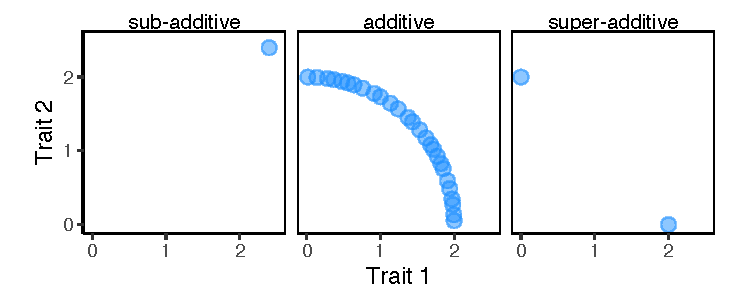
\includegraphics{1-outcomes_q2.pdf}
\caption{Unique trait values for surviving species in simulations of 2-trait communities,
    for tradeoffs being sub-additive ($\eta < 0$), additive ($\eta = 0$), or 
    super-additive ($\eta > 0$).}
\label{fig:two-trait-outcomes}
\end{figure}




The proportion of the 100 species introduced to communities that survived and
coexisted depended on the additive genetic variance, 
the non-additive tradeoffs, and 
how conflicting / non-conflicting evolution was (i.e., the values of $d_1$ 
and $d_2$) (Figure \ref{fig:coexistence-spp}A).
Greater additive genetic variance increased the probability of evolutionary 
rescue, where species evolved quickly enough towards a fitness peak to
prevent themselves from going extinct.
Sub-additive tradeoffs resulted in greater numbers of species because
the lower cost of evolving multiple traits caused species to evolve
high values of both traits.
When combined with non-conflicting evolution,
this decreased competition experienced by all species, both on a 
per-capita basis (the term $- \mathbf{v}_{j}^{\text{T}} \mathbf{D} \mathbf{v}_j$ 
in equation \ref{eq:competition})
and overall (because all $N_j$ are greater).
Increasing $d_1$ and $d_2$ caused greater number of species to coexist
because species evolving toward a fitness peak benefited rather than 
harmed other species with high $d_1$ and $d_2$.
There was an abrupt change when evolution was conflicting for both traits 
(i.e., $d_1 < 0$ and $d_2 < 0$),
where only one species ever survived.

When we kept evolution for the first trait non-conflicting ($d_1 = 0.1$) and
adjusted evolution for trait 2, the results were slightly more complicated
(Figure \ref{fig:coexistence-spp}B).
Additive genetic variance had a similar effect as when we varied both traits' evolution.
The effect of varying $d_1$, however, depended on the tradeoffs.
With sub-additive tradeoffs, the threshold for coexistence was $d_1 = -0.1$.
This is because species evolve to maximize both traits, so $d_1 + d_2$
determines the coexistence behavior of the community.
When tradeoffs are super-additive, $\min (d_1, d_2)$ determines whether 
coexistence can occur.
This is because under super-additivity, species evolve to maximize one trait while 
the other evolves to zero.
When one $d$ is negative, if sufficient species are added to the community and 
each starts with random trait values, 
one will inevitably evolve to maximize the trait that is conflicting. 
That species will exclude all others.


\begin{figure}[ht!]
\centering
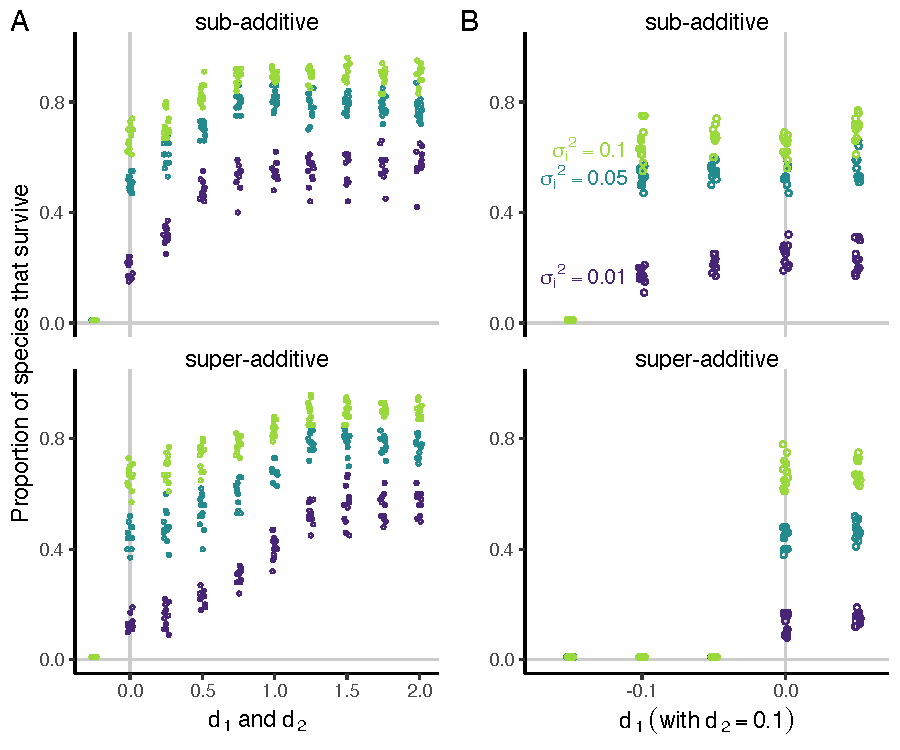
\includegraphics{2-coexist_spp.pdf}
\caption{Proportion of species that survived in simulations of 100-species, 2-trait
    communities with varying additive genetic variances ($\sigma_i^2$), and 
    varying (A) $d_1$ and $d_2$ or (B) varying $d_1$ with $d_2$ fixed at 0.1.
    Shown are both sub-additive ($\eta < 0$) or super-additive ($\eta > 0$) tradeoffs.}
\label{fig:coexistence-spp}
\end{figure}




% ------------------------------------------------------------------------------
% ------------------------------------------------------------------------------
% ------------------------------------------------------------------------------
% ------------------------------------------------------------------------------
% 
% LEFT OFF HERE
% 
% ------------------------------------------------------------------------------
% ------------------------------------------------------------------------------
% ------------------------------------------------------------------------------
% ------------------------------------------------------------------------------



\ref{fig:conditional-coexistence}


\begin{figure}[ht!]
\centering
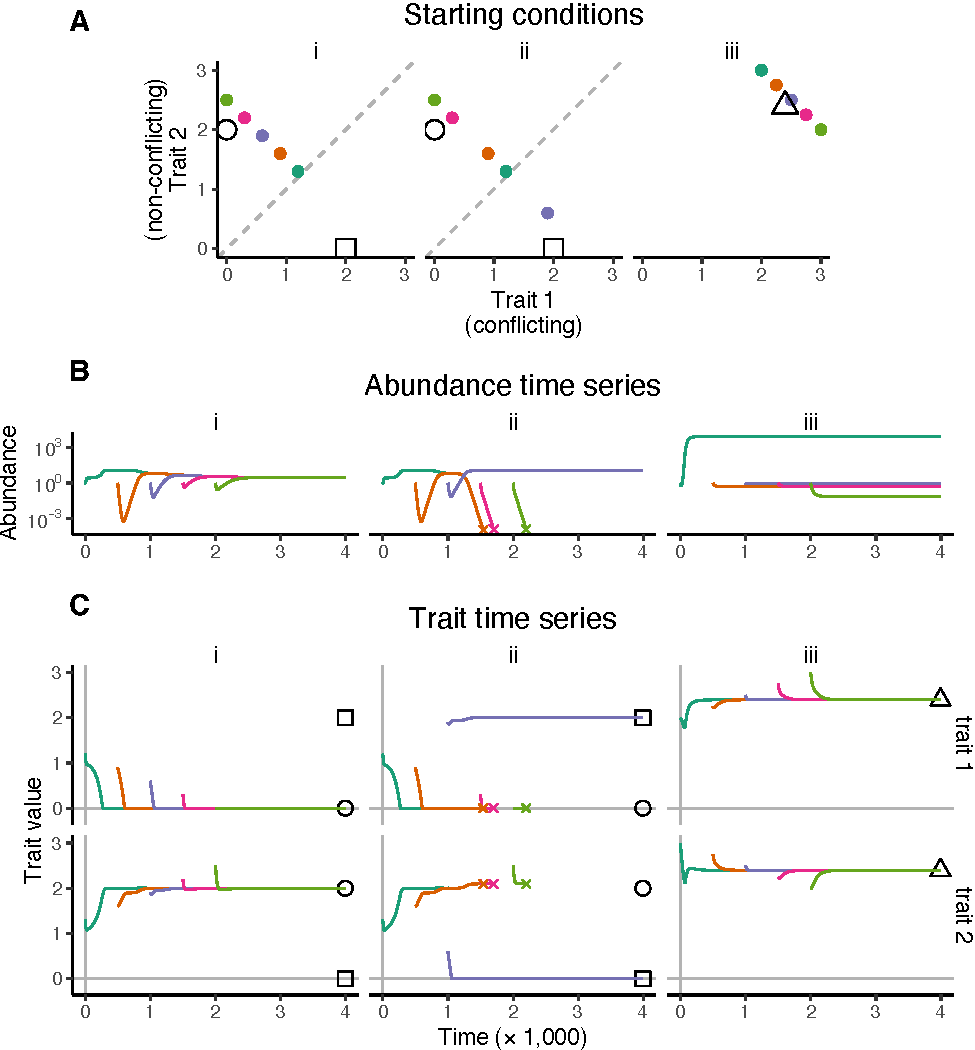
\includegraphics{3-cond_coexist_conflicting.pdf}
\caption{Conditional coexistence for 2-trait, 5-species communities when trait 1 has 
    conflicting evolution and trait 2 has non-conflicting.
    Panels show, for each of three situations,
    (A) starting conditions for each species in trait space, 
    (B) abundances through time, and 
    (C) trait values through time.
    Situations i and ii have super-additive tradeoffs, while situation iii has 
    sub-additive.
    In (A), the dotted line separates the basins of attraction for the two possible
    trait states.
    In (A,C), shapes of hollow points indicate the equilibrium trait state.
    In (B,C), Xs mark extinction events.
}
\label{fig:conditional-coexistence}
\end{figure}










Super-additivity can lead to multiple possible trait states in a 
community.
When species start with trait values that vary widely 
across the trait space, both trait states can be occupied 
simultaneously only when evolution for both traits is non-conflicting.
However, when one trait is non-conflicting and all starting
trait values in the community lie in the basin of attraction
for that trait being maximized, then coexistence can occur
(Figure \ref{fig:cond-coexist}).
Thus, even in this simple case, community evolution can follow
one of two paths depending on starting conditions:
One species evolves fastest to the conflicting state and 
excludes others, or
multiple species evolve to the non-conflicting state
and coexist.







% ---------------------------------------------------------------------------------------
% ---------------------------------------------------------------------------------------
% Discussion
% ---------------------------------------------------------------------------------------
% ---------------------------------------------------------------------------------------

\section*{Discussion}




\section*{Conclusion}



% ---------------------------------------------------------------------------------------
% ---------------------------------------------------------------------------------------
% Acknowledgments
% ---------------------------------------------------------------------------------------
% ---------------------------------------------------------------------------------------
% You may wish to remove the Acknowledgments section while your paper
% is under review (unless you wish to waive your anonymity under
% double-blind review) if the Acknowledgments reveal your identity.
% If you remove this section, you will need to add it back in to your
% final files after acceptance.

% \section*{Acknowledgments}
%
% OEC would like to thank the world. GHC is much indebted to the solar system. AQE was supported by a generous grant from the Milky Way (MW/01010/987654).


% ---------------------------------------------------------------------------------------
% ---------------------------------------------------------------------------------------
% Appendix A and B
% ---------------------------------------------------------------------------------------
% ---------------------------------------------------------------------------------------

\clearpage

\renewcommand{\thefigure}{A\arabic{figure}}
\renewcommand{\theequation}{A\arabic{equation}}
\renewcommand{\thetable}{A\arabic{table}}
\setcounter{equation}{0}
\setcounter{figure}{0}
\setcounter{table}{0}


\section*{Appendix A: Matrix derivatives in quantitative genetics equations}


% In this section, we make the following abbreviation in the equations:

% \begin{equation*}
%     \mathbf{\Omega}_{i,t} \equiv N_{i,t} +
%             \sum_{j \ne i}^{n}{ N_{j,t} \, \textrm{e}^{
%             - \mathbf{v}_{j,t}^{\textrm{T}}
%             \mathbf{D} \mathbf{v}_{j,t} } }
% \end{equation*}

\subsection*{Axis change}

The partial derivative of fitness with respect to axes is

\begin{equation*}
\begin{split}
    \frac{ \partial F_{i,t} }{ \partial \mathbf{v}_{i,t} } =
        \exp & \left\{
            r_0
            - f \mathbf{v}_{i,t}^{\textrm{T}} \mathbf{C} \mathbf{v}_{i,t}
            - \alpha_0  \left(
                N_{i,t} + \sum_{j \ne i}^{n}{ N_{j,t} \, \textrm{e}^{
                - \mathbf{v}_{j,t}^{\textrm{T}}
                \mathbf{D} \mathbf{v}_{j,t} } }
            \right) \,
                \textrm{e}^{- \mathbf{v}_{i,t}^{\textrm{T}} \mathbf{v}_{i,t}}
        \right\} \\
        & \left[
            2 \alpha_0 \left(
                N_{i,t} + \sum_{j \ne i}^{n}{ N_{j,t} \, \textrm{e}^{
                - \mathbf{v}_{j,t}^{\textrm{T}}
                \mathbf{D} \mathbf{v}_{j,t} } }
            \right) \,
                \textrm{e}^{- \mathbf{v}_{i,t}^{\textrm{T}} \mathbf{v}_{i,t}} \:
                \mathbf{v}_{i,t}^{\textrm{T}}
            - 2 f \mathbf{v}_{i,t}^{\textrm{T}} \mathbf{C}
        \right]
    \textrm{.}
\end{split}
\end{equation*}


This, combined with equation \ref{eq:axis-change}, means that axes change as follows:

\begin{equation} \label{eq:axes-change-full}
    \mathbf{v}_{i,t+1} = \mathbf{v}_{i,t} + 2 \sigma_i^2
    \left[
        \alpha_0 \, \left(
            N_{i,t} +
            \sum_{j \ne i}^{n}{ N_{j,t} \, \textrm{e}^{
            - \mathbf{v}_{j,t}^{\textrm{T}}
            \mathbf{D} \mathbf{v}_{j,t} } }
        \right) \:
            \textrm{e}^{- \mathbf{v}_{i,t}^{\textrm{T}} \mathbf{v}_{i,t}} \:
            \mathbf{v}_{i,t}^{\textrm{T}}
        - f \, \mathbf{v}_{i,t}^{\textrm{T}} \: \mathbf{C}
    \right]
    \textrm{.}
\end{equation}


\subsection*{Jacobian}

The Jacobian is made up of the following derivatives:

\begin{equation*}
\begin{split}
    \frac{ \partial \, \mathbf{v}_{i,t+1} }{ \partial \, \mathbf{v}_{i,t} } &= 
    \mathbf{I} + 2 ~ \sigma_i^2 ~
        \left[
            \alpha_0 ~ \left(
                N_{i,t} + \sum_{j \ne i}^{n}{ N_{j,t} \, \textrm{e}^{
                - \mathbf{v}_{j,t}^{\textrm{T}}
                \mathbf{D} \mathbf{v}_{j,t} } }
            \right) ~ \textrm{e}^{ - \mathbf{v}_{i,t}^{\textrm{T}} \mathbf{v}_{i,t} }
            \left(
                \mathbf{I} - 2 ~ \mathbf{v}_{i,t} \mathbf{v}_{i,t}^{\textrm{T}}
            \right) -
            f \: \mathbf{C}^{\textrm{T}}
        \right] \\
    \frac{ \partial \: \mathbf{v}_{i,t+1} }{ \partial \: \mathbf{v}_{k,t}} &=
        -4 \; \sigma_i^2 \; \alpha_0 \; N_{k,t} \; \mathbf{v}_{i,t} \;
        \textrm{e}^{
                    - \mathbf{v}_{k,t}^{\textrm{T}} \mathbf{D} \mathbf{v}_{k,t}
                    - \mathbf{v}_{i,t}^{\textrm{T}} \mathbf{v}_{i,t}
                } \;
        \mathbf{v}_{k,t}^{\textrm{T}} \; \mathbf{D} \\
% 
    \frac{ \partial \: \mathbf{v}_{i,t+1} }{ \partial \: N_{i,t} } &=
        2 \; \sigma_i^2 \; \alpha_0 \; \mathbf{v}_{i,t} \;
        \textrm{e}^{ - \mathbf{v}_{i,t}^{\textrm{T}} \mathbf{v}_{i,t} } \\
    \frac{ \partial \: \mathbf{v}_{i,t+1} }{ \partial \: N_{k,t} } &=
        2 \; \sigma_i^2 \; \alpha_0 \; \mathbf{v}_{i,t} \;
        \textrm{e}^{ - \mathbf{v}_{k,t}^{\textrm{T}} \mathbf{D} \mathbf{v}_{k,t}
            - \mathbf{v}_{i,t}^{\textrm{T}} \mathbf{v}_{i,t} } \\
% 
    \frac{ \partial N_{i,t+1} }{ \partial \mathbf{v}_{i,t} } &= 
        2 \, F_{i,t+1} \,  N_{i,t}
        \left[
            \alpha_0 \, \left(
                N_{i,t} + \sum_{j \ne i}^{n}{ N_{j,t} \, \textrm{e}^{
                - \mathbf{v}_{j,t}^{\textrm{T}}
                \mathbf{D} \mathbf{v}_{j,t} } }
            \right) \, \text{e}^{ -\mathbf{v}_{i,t}^{\text{T}}
            \mathbf{v}_{i,t} } \, \mathbf{v}_{i,t}^{\text{T}}
            - f \, \mathbf{v}_{i,t}^{\text{T}} \, \mathbf{C}
        \right] \\
    \frac{ \partial N_{i,t+1} }{ \partial \mathbf{v}_{k,t} } &= 
        2 \, F_{i,t+1} \, N_{i,t} \, N_{k,t} \, \alpha_0 \: 
        \text{e}^{ -\mathbf{v}_{i,t}^{\text{T}} \mathbf{v}_{i,t} -
            \mathbf{v}_{k,t}^{\text{T}} \mathbf{D} \mathbf{v}_{k,t} } \:
        \mathbf{v}_{k,t}^{\text{T}} \, \mathbf{D} \\
% 
    \frac{ \partial N_{i,t+1} }{ \partial N_{i,t} } &= 
        F_{i,t+1}
        \left(
            1 - N_{i,t} \: \alpha_0 \: 
            \text{e}^{ -\mathbf{v}_{i,t}^{\text{T}} \mathbf{v}_{i,t} } 
        \right) \\
    \frac{ \partial N_{i,t+1} }{ \partial N_{k,t} } &= 
        - F_{i,t+1} \: N_{i,t} \: \alpha_0 \: 
        \text{e}^{ -\mathbf{v}_{i,t}^{\text{T}} \mathbf{v}_{i,t} -
            \mathbf{v}_{k,t}^{\text{T}} \mathbf{D} \mathbf{v}_{k,t} } 
    \textrm{.}
\end{split}
\end{equation*}



\subsection*{Keeping axes non-negative}

To keep axes $\ge 0$, we used the ramp function, $R(x)$, which is defined as

\begin{equation*}
    R(x) = \begin{cases}
        x & \text{if}\ x \ge 0 \\
        0 & \text{if}\ x < 0
        \end{cases}
    \text{.}
\end{equation*}


\noindent Its derivative is the Heaviside step function:

\begin{equation*}
\begin{split}
    R'(x) &= H(x) \\
    H(x) &= \begin{cases}
        0 & \text{if}\ x \le 0 \\
        1 & \text{if}\ x > 0
        \end{cases}
    \text{.}
\end{split}
\end{equation*}

% Also see https://see.stanford.edu/materials/lsoftaee261/book-fall-07.pdf
% and https://mathworld.wolfram.com/RampFunction.html

Thus, all axis derivatives of the form $\partial \mathbf{v} / \partial x$
are changed to $H(\mathbf{v}(x)) \: \partial \mathbf{v} / \partial x$ to 
account for axes being non-negative.



\clearpage

\renewcommand{\thefigure}{B\arabic{figure}}
\renewcommand{\theequation}{B\arabic{equation}}
\renewcommand{\thetable}{B\arabic{table}}
\setcounter{equation}{0}
\setcounter{figure}{0}
\setcounter{table}{0}


\section*{Appendix B: Two-axis solutions}



\subsection*{Effects of stochasticity on axis evolution}

When there is stochasticity in axis evolution,
the second order Taylor series approximation for the expected
value of axis 1 at time $t+1$ is

\begin{equation}
\label{eq:taylor-expansion-final}
\begin{split}
    \text{E}(v_{1,t+1}) \approx
        v_{1,t} + 2 \; \sigma_A^2 \Bigg\{ 
            & \alpha_0 \; \Omega \; v_{1,t} \; \text{e}^{-v_{1,t}^2 - v_{2,t}^2} 
            \bigg[ 
                1 + \sigma^2_{\varepsilon_1} \left( \frac{1}{2} - 4 \; v_{1,t}^2 \right)
                - 2 \; \sigma^2_{\varepsilon_2} \, v_{2,t}^2 \left( 1 - v_{2,t}^2 \right)
            \bigg] \\
            & - f \bigg[
                v_{1,t} + \eta \; v_{2,t} + \frac{1}{2} \left(
                    \sigma^2_{\varepsilon_1} \, v_{1,t} + \sigma^2_{\varepsilon_2} \, \eta \; v_{2,t}
                \right)
            \bigg]
        \Bigg\}
\text{,}
\end{split}
\end{equation}

where we drop the index for species to reduce clutter.
Subscripts for axes are reversed for the approximation for axis 2.






\clearpage
\section*{Appendix C: Supplemental Figures}

\renewcommand{\thefigure}{C\arabic{figure}}
\renewcommand{\theequation}{C\arabic{equation}}
\renewcommand{\thetable}{C\arabic{table}}
\setcounter{equation}{0}
\setcounter{figure}{0}
\setcounter{table}{0}



\begin{figure}[ht!]
\centering
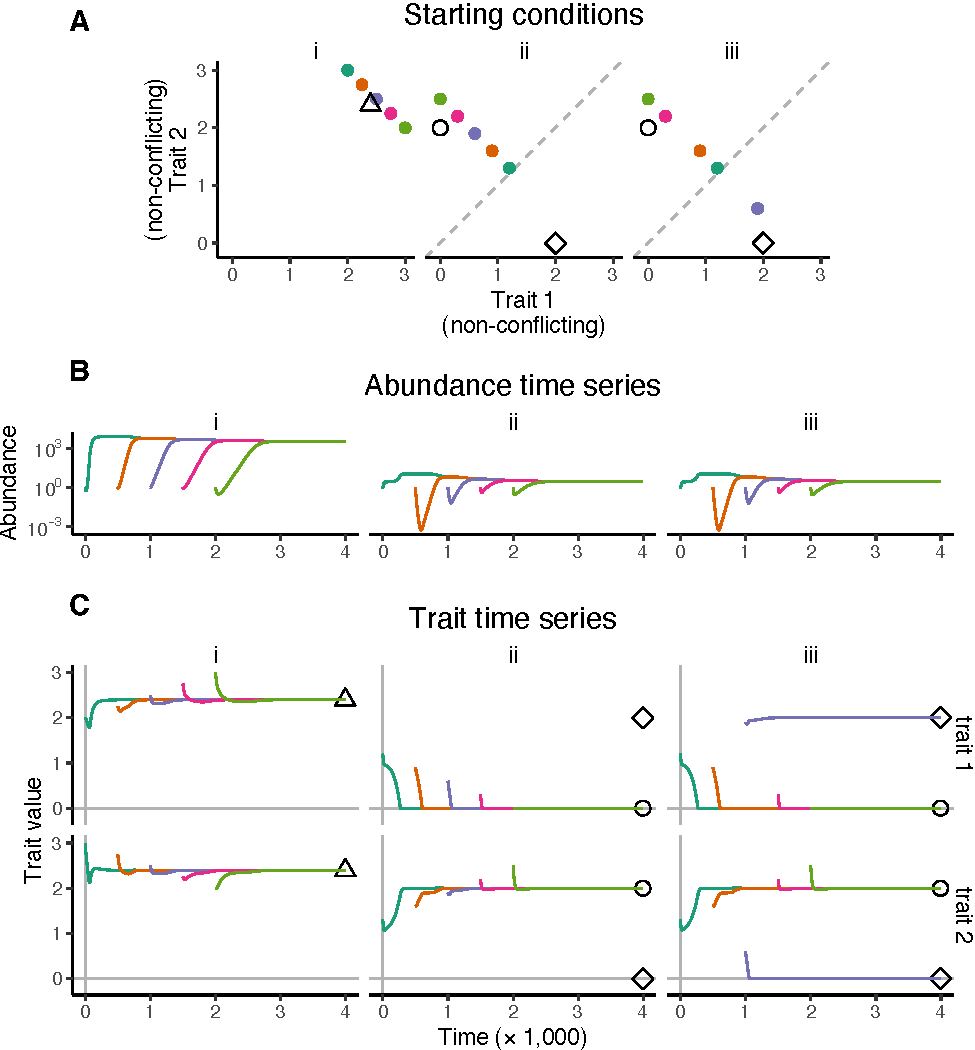
\includegraphics[width=\textwidth]{S1-cond_coexist_non-conflicting.pdf}
% \caption{Number of surviving species for 24 simulations of 2-trait 
%     communities
%     (A) after 50,000 generations for all permutations of the traits
%     being conflicting (``$-$'') or non-conflicting (``$+$''),
%     (B) after 50,000 generations for varying values of $d_2$ when 
%     $d_1$ is kept positive (i.e., trait 1 is kept non-conflicting), and
%     (C) through time with $d_2 = -10^{-2}$ and $d_2 = -10^{-4}$.
%     For all panels, $d_1 = 0.05$, $\eta = 0.6$, and species start with
%     random trait values ($\sim \text{N}(0,2)$ truncated $> 0$).
%     In (A), $d_2 = 0.1$.}
\caption{}
\label{fig:cond-coexist-non-conflicting}
\end{figure}


% \begin{figure}[ht!]
% \centering
% 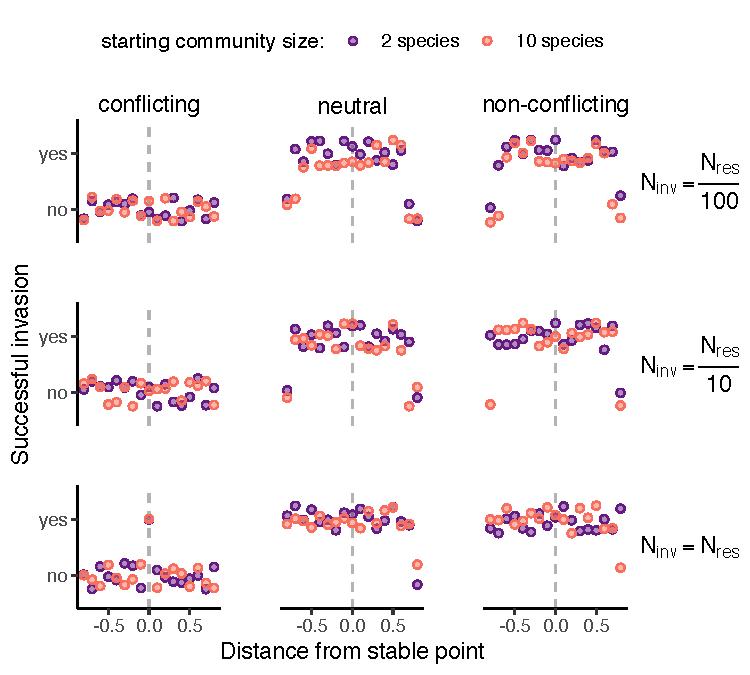
\includegraphics{S2-invasion.pdf}
% \caption{Invasion success for a 2-trait equilibrium community based on
%     the invader's starting distance from the equilibrium point in trait space.
%     Sub-panel columns indicate the type of evolution.
%     Sub-panels rows indicate the invaders' starting
%     abundances ($N_{eq}$) in relation to the residents'
%     abundances ($N_{res}$); all residents had the same
%     abundance.
%     Point color indicates the size of the resident community.
%     In these simulations, the resident community all had
%     trait values based on the analytical solutions for equilibria
%     in Appendix B.
%     The single invading species always had its first trait start
%     at the equilibrium value, but its second trait 
%     varied from
%     $-0.8$ to $0.8$ from the equilibrium value.
%     Simulations ran for 50,000 generations and assessed invasion 
%     success as the presence of the invader.
%     Here, $\eta = -0.6$, $d \in \{ -0.01, \; 0, \; 0.01 \}$.
% }
% \label{fig:invasion}
% \end{figure}

\begin{figure}[ht!]
\centering
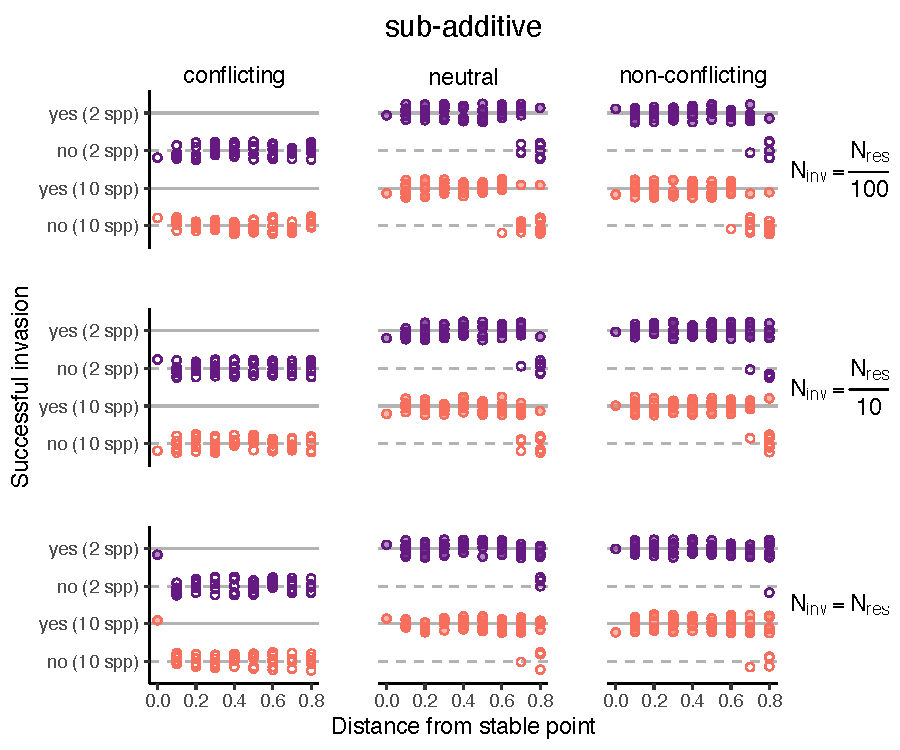
\includegraphics{S2-invasion_sub.pdf}
\caption{}
\label{fig:invasion-sub}
\end{figure}


\begin{figure}[ht!]
\centering
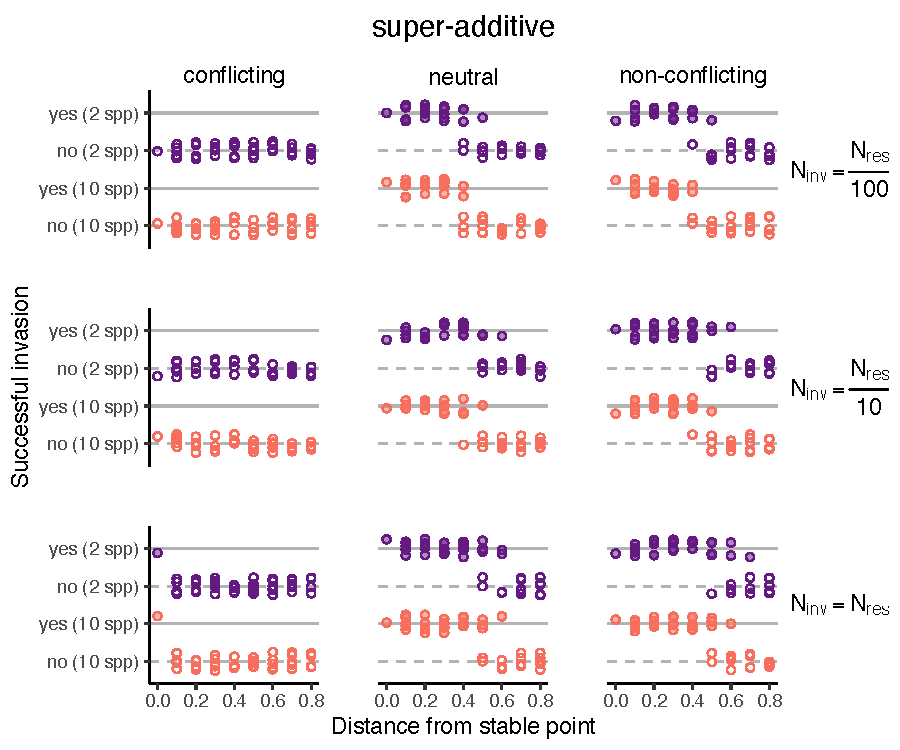
\includegraphics{S3-invasion_super.pdf}
\caption{}
\label{fig:invasion-super}
\end{figure}


% \clearpage
% \section*{Appendix D: Four-trait equilibrium solutions}

\renewcommand{\thefigure}{D\arabic{figure}}
\renewcommand{\theequation}{D\arabic{equation}}
\renewcommand{\thetable}{D\arabic{table}}
\setcounter{equation}{0}
\setcounter{figure}{0}
\setcounter{table}{0}



I haven't done these.




% ---------------------------------------------------------------------------------------
% ---------------------------------------------------------------------------------------
% Literature Cited
% ---------------------------------------------------------------------------------------
% ---------------------------------------------------------------------------------------



\bibliographystyle{amnatnat.bst}
\clearpage
\bibliography{refs.bib}

\end{document}
